\section{Introduction}
\label{sec:intro}
Face verification is used to unlock phones, authorize payments and control access. Deep verification models compare the embeddings of two images, and it is well known that small, almost invisible perturbations can make them accept an impostor or reject the genuine user~\cite{goswami2018unravelling}. Robust training is effective but costly, and many deployed systems instead rely on lightweight preprocessing such as JPEG compression~\cite{dziugaite2016jpeg,das2018shield}. The difficulty is that preprocessing defenses are often evaluated against attacks that ignore them; once the attacker approximates the defense, protection largely disappears~\cite{athalye2018obfuscated}.

\paragraph{Question.} Can a lightweight defense reduce attacks on face verification while preserving clean accuracy \emph{when the attacker knows the defense}?

\paragraph{Approach.} We keep the pretrained embedder frozen and add (i) a bank of cheap transformations used as a consistency check and (ii) a small classifier on the resulting features, fused with the verification score by a Bayes minimum-risk rule (Fig.~\ref{fig:pipeline}). The idea follows feature squeezing~\cite{xu2018squeeze}, adapted to verification \emph{pairs} and to a three-way decision that includes a Flag output.

\paragraph{Contributions.} (1) A reproducible, identity-disjoint evaluation protocol on LFW with FGSM, PGD, DeepFool, CW, Square and adaptive BPDA attacks. (2) A side-by-side comparison of non-adaptive and adaptive attacks against JPEG, Gaussian, median and bit-depth defenses. (3) A transformation-consistency detector with Bayes fusion, evaluated on seen and unseen attacks, other budgets, benign controls, ablations and cost. We state clearly what does \emph{not} work (Square) and what is not established (worst-case adaptive robustness).

\begin{figure*}[t]
  \centering
  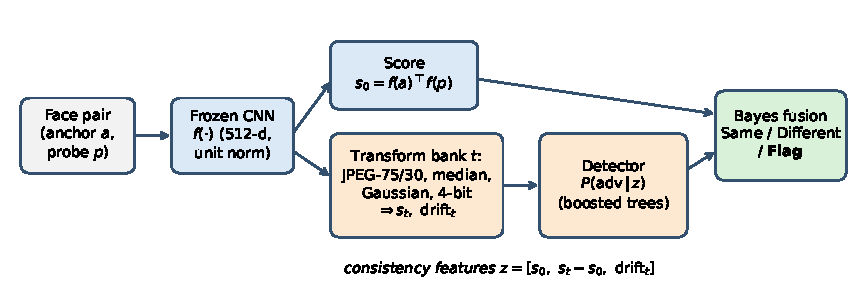
\includegraphics[width=0.92\linewidth]{figures/pipeline.pdf}
  \caption{Proposed pipeline. A frozen CNN embeds both images; the same pair is re-embedded under cheap transformations; the score and drift features feed a clean-vs-attacked detector whose posterior is fused with the verification score (Bayes minimum risk) into Same / Different / Flag.}
  \label{fig:pipeline}
\end{figure*}
